\documentclass[a4paper,11pt]{report}
\usepackage[T1]{fontenc}
\usepackage[utf8]{inputenc}
\usepackage{lmodern}
\usepackage[english]{babel}
\usepackage{amsfonts}
\usepackage{hyperref}
\usepackage{graphicx}
\usepackage{subcaption}

\title{Technical report from 08/01/2014 to 31/01/2014}
\author{Rafael Reggiani Manzo}

\begin{document}

\maketitle
\tableofcontents

\begin{abstract}
  This document is intended to make easier for me to explain on what I've been working on, as well as remembering about last meetings and objectives.

  This time I've computed the same statistics from previous meetings, but just for the \textit{corpus callosum} region, expecting to see something visually meaningful.
\end{abstract}

\chapter{Previous meeting}
Here follows a brief recapitulation from our last meeting on 08/01/2014.

  \section{What was presented}
  Last time where presented statistics (mean and standard deviation for MD, FA, RD, TC and TV values) for the whole brain filtered out voxels with FA value below 0.2. Then where applied four clustering criterias (by FA, RD, TC or TV values) and for each clustered voxel recalculated the statistics. Finally were produced histograms of the distribution of cluster count according to it's MD, FA, RD, TC and TV mean values.

  \section{Next steps}
  Unfortunately, with the data produced was not possible to produce any kind of classification or conclude anything. This was in part consequence of the size of the region analyzed and in part because of the lack of a image with each clustered region colored and identified and some of the histogram labels unreadable.

  So the objective now was to repeat the process but with a restricted brain structure, the \textit{corpus callosum}, and produce the expected visual representations.

  Further, in order to conclusively study tractography through uncertainty regions, a dataset extracted from a well known phantom will of great value. So, I've started with a first sketch from what I think would be useful.

\chapter{Work done}

  \section{\textit{Corpus callosum} structure}
  Since I was focusing the work specifically on this region of the brain, I've decided that would be useful to learn more about its anatomy. To do so, I've read the following article about the fibers composing it: \textit{F. Aboitiz, A. B. Scheibel, R. S. Fisher, and E. Zaidel, Fiber composition of the human corpus callosum," Brain Res, vol. 598, pp. 143-53, Dec 1992.}

  After reading there was no knowledge that I could apply right now, but of course it was full of informations about axon diameters, fiber types and for example how the \textit{corpus callosum} is responsible for interhemispheric transfer.

  \section{Regions and statistics}
  The following statistics refer to the high resolution dataset with a mask restrained to the \textit{corpus callosum} region with it's fibers expanded using the adaptive Runge-Kutta method.

  First I'll present the statistics for the dataset with voxels with FA values under 0.2 which was the base for the clustering which I'll present just after.

    \newpage
    \subsection{FA threshold}\label{subsec:fa-threshold}

    \begin{figure}[!ht]
      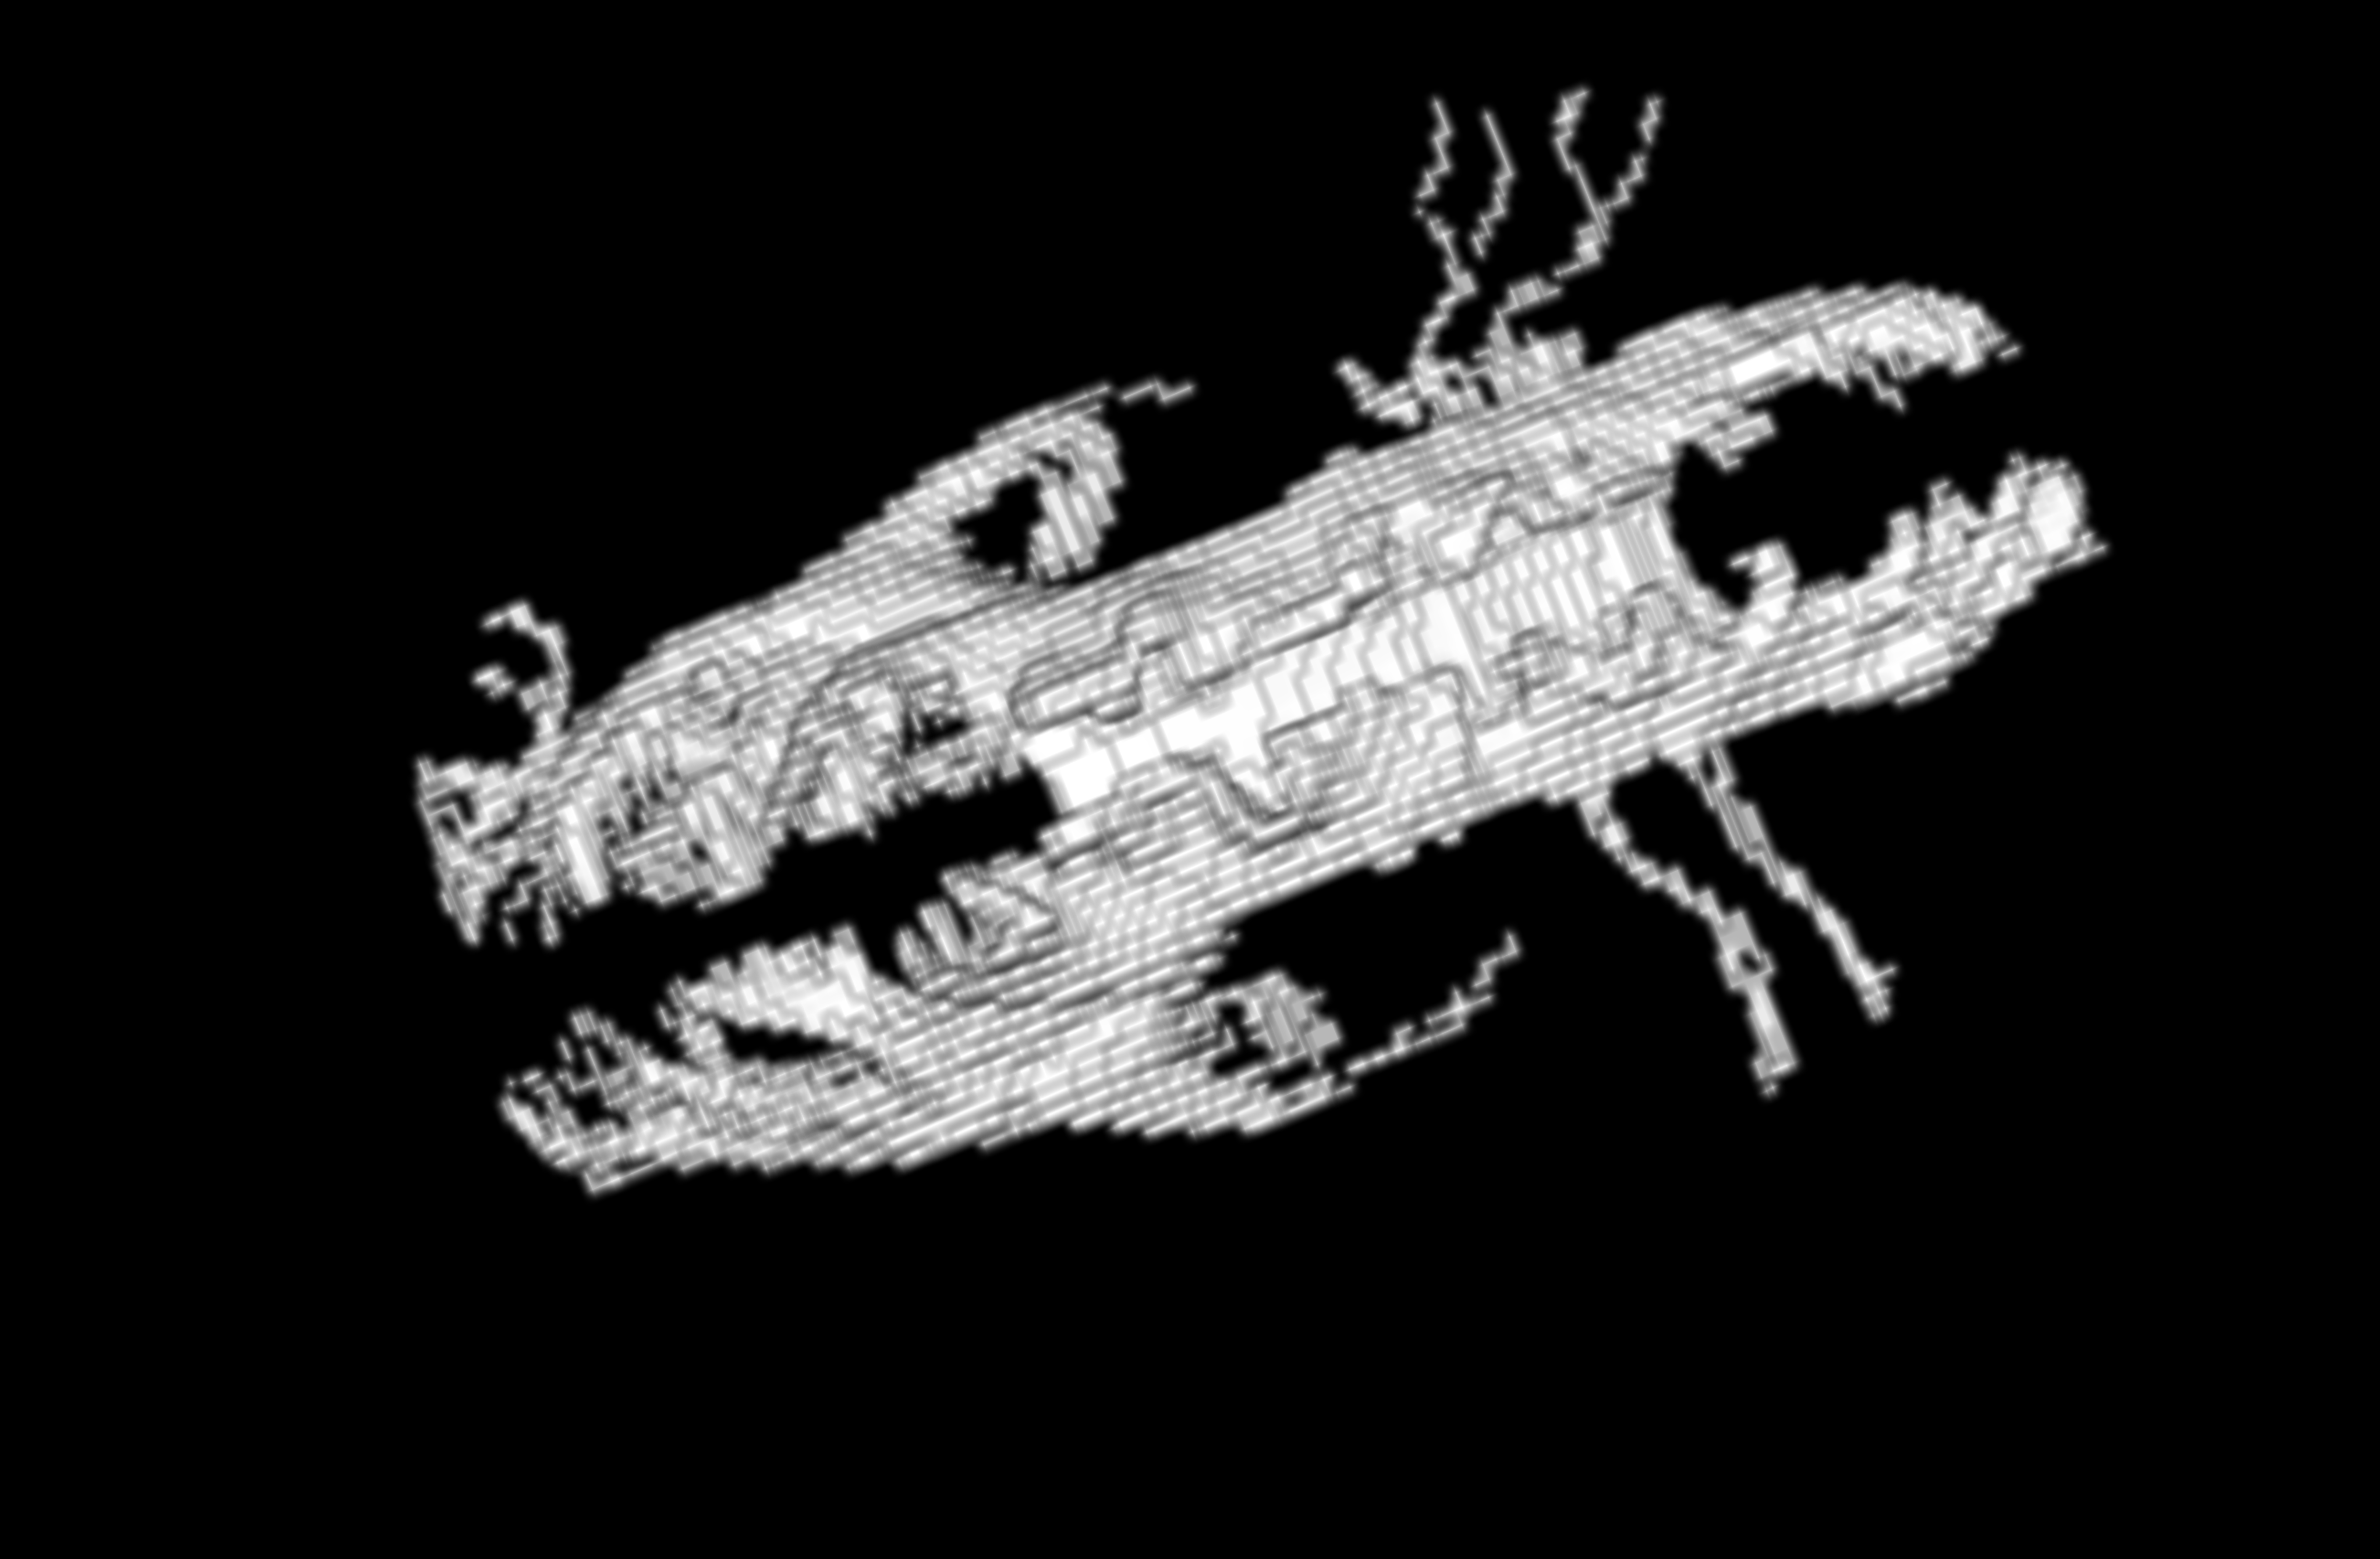
\includegraphics[width=1\linewidth]{img/regions/whole.png}
      \caption{3D view of \textit{corpus callosum} with fibers tracked by the adaptive Runge-Kutta algorithm on Bio Image Suite.}
      \label{fig:whole}
    \end{figure}

    The image \ref{fig:whole} represents the region for which were extracted the regions below and, afterwards, for which the clustering algorithms were applied.

    After the threshold filter there were 21041 voxels left in the dataset. The time taken to generate the mask was 0m7.496s and the statistics calculation took 1m22.496s.

    \begin{tabular}{| c | c | c | c | c | c |}
      \hline
        & \textbf{MD} & \textbf{FA} & \textbf{RD} & \textbf{TV} & \textbf{TC} \\ \hline
       \textbf{Mean} & 0.0001583 & 0.4651988 & 0.0001146 & 0.0000010 & 0.0000001 \\ \hline
       \textbf{Standard Deviation} & 0.000025 & 0.1229444 & 0.0000292 & 0.00000001 & 0.0000004 \\ \hline 
    \end{tabular}

    \subsection{Clustering}\label{subsec:clustering}
    In order to get closer to identify a pattern to apply the clustering for each tensor metric and then look at their mean and standard deviation.

    Beyond the results, following I'll also mention the processing time taken to produce those results. For this I've used a Intel Core 2 Due E7400 with 2 physical cores at 2.8 GHz.

    The applied clustering algorithm was DBSCAN\footnote{as described in: Domenica Arlia and Massimo Coppola. 2001. Experiments in Parallel Clustering with DBSCAN. In Proceedings of the 7th International Euro-Par Conference Manchester on Parallel Processing (Euro-Par '01), Rizos Sakellariou, John Keane, John R. Gurd, and Len Freeman (Eds.). Springer-Verlag, London, UK, UK, 326-331.} with 1 one voxel neighbourhood length and one point was not considered noise if it had at least 26 neighbours.

    \newpage
    \subsubsection{FA}
    \begin{figure}[!ht]
      \centering

      \begin{subfigure}[t]{.49\textwidth}
        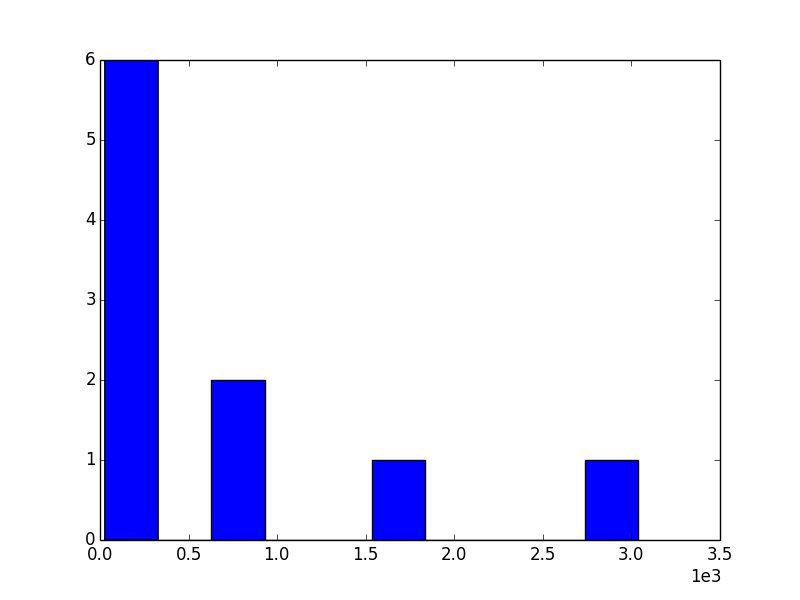
\includegraphics[width=1\linewidth]{img/histograms/fa_clustered_fa_mask_region_sizes_hist.png}
        \caption{Cluster size distribution histogram (Voxel count X Cluster count).}
        \label{subfig:fa_hist_region}
      \end{subfigure}\hfill%
      \begin{subfigure}[t]{.49\textwidth}
        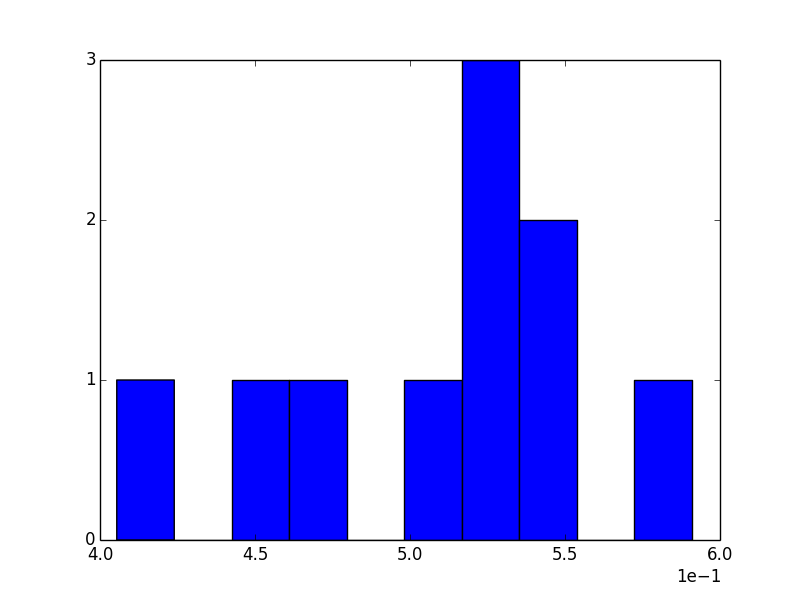
\includegraphics[width=1\linewidth]{img/histograms/fa_clustered_fa_mask_fa_means_hist.png}
        \caption{Histogram for FA mean frequency (Cluster count X FA mean).}
        \label{subfig:fa_hist_fa}
      \end{subfigure}\hfill\\
      \begin{subfigure}[t]{.49\textwidth}
        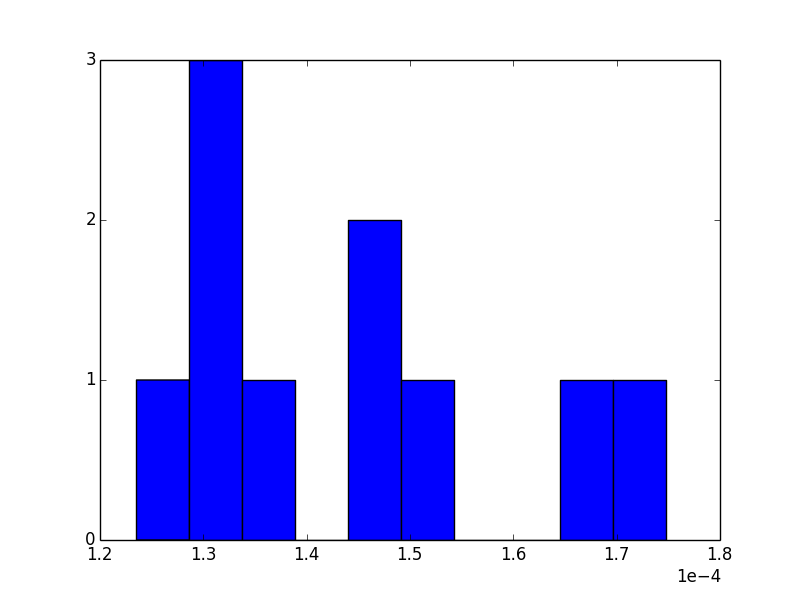
\includegraphics[width=1\linewidth]{img/histograms/fa_clustered_fa_mask_md_means_hist.png}
        \caption{Histogram for MD mean frequency (Cluster count X MD mean).}
        \label{subfig:fa_hist_md}
      \end{subfigure}\hfill%
      \begin{subfigure}[t]{.49\textwidth}
        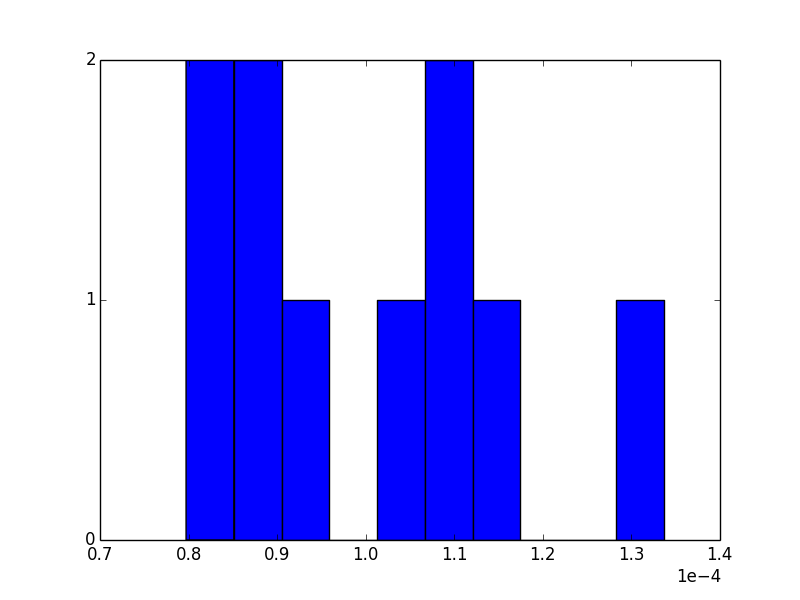
\includegraphics[width=1\linewidth]{img/histograms/fa_clustered_fa_mask_rd_means_hist.png}
        \caption{Histogram for RD mean frequency (Cluster count X RD mean).}
        \label{subfig:fa_hist_rd}
      \end{subfigure}\hfill\\
      \begin{subfigure}[t]{.49\textwidth}
        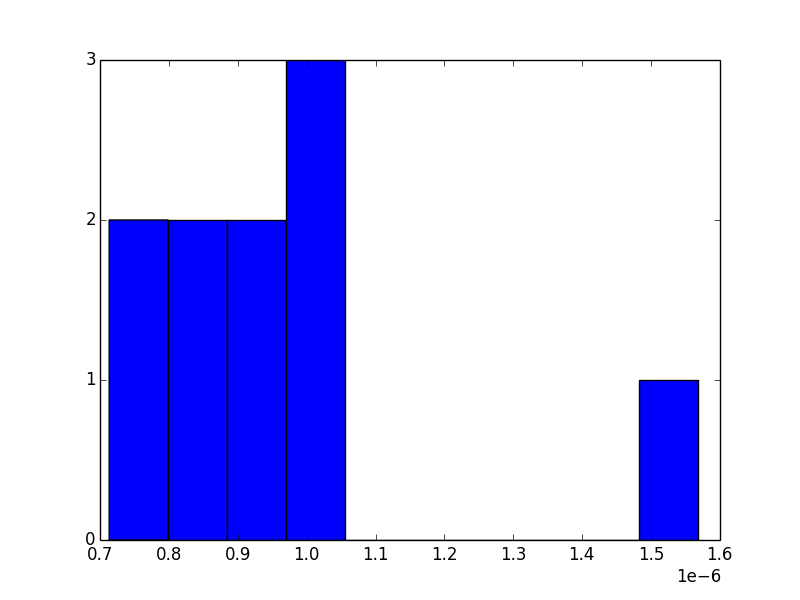
\includegraphics[width=1\linewidth]{img/histograms/fa_clustered_fa_mask_tc_means_hist.png}
        \caption{Histogram for TC mean frequency (Cluster count X TC mean).}
        \label{subfig:fa_hist_tc}
      \end{subfigure}\hfill%
      \begin{subfigure}[t]{.49\textwidth}
        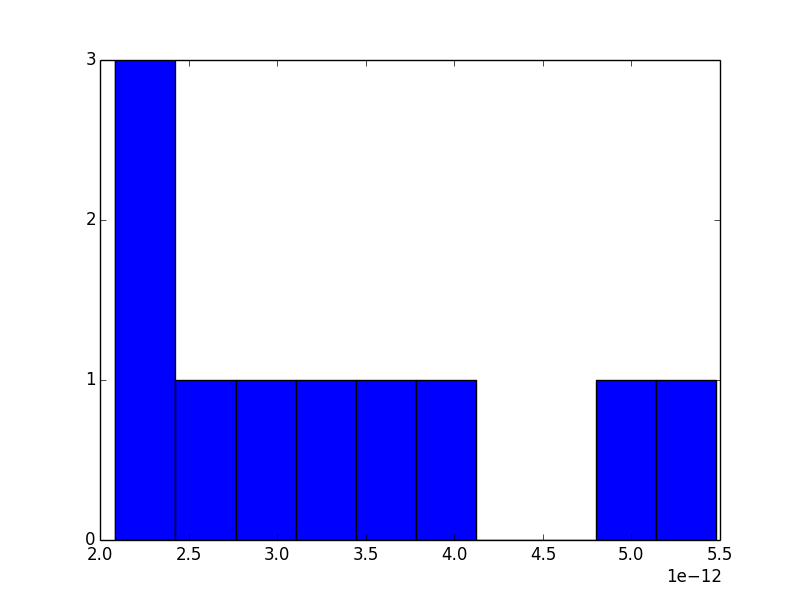
\includegraphics[width=1\linewidth]{img/histograms/fa_clustered_fa_mask_tv_means_hist.png}
        \caption{Histogram for TV mean frequency (Cluster count X TV mean).}
        \label{subfig:fa_hist_tv}
      \end{subfigure}\hfill

      \caption{Histograms for statistics distribution when clustered by FA values.}
      \label{fig:fa-histograms}
    \end{figure}

    This type of clusterization grouped voxels with FA values which don't differ no more then 0.246 (twice the standard deviation from the entire region \ref{subsec:fa-threshold}) taking 8m16.831s to get computed and another 0m25.687s to generate the statistics.

    Those statistics refers to the following colored regions on \ref{fig:fa-regions}.

    \begin{figure}[!ht]
      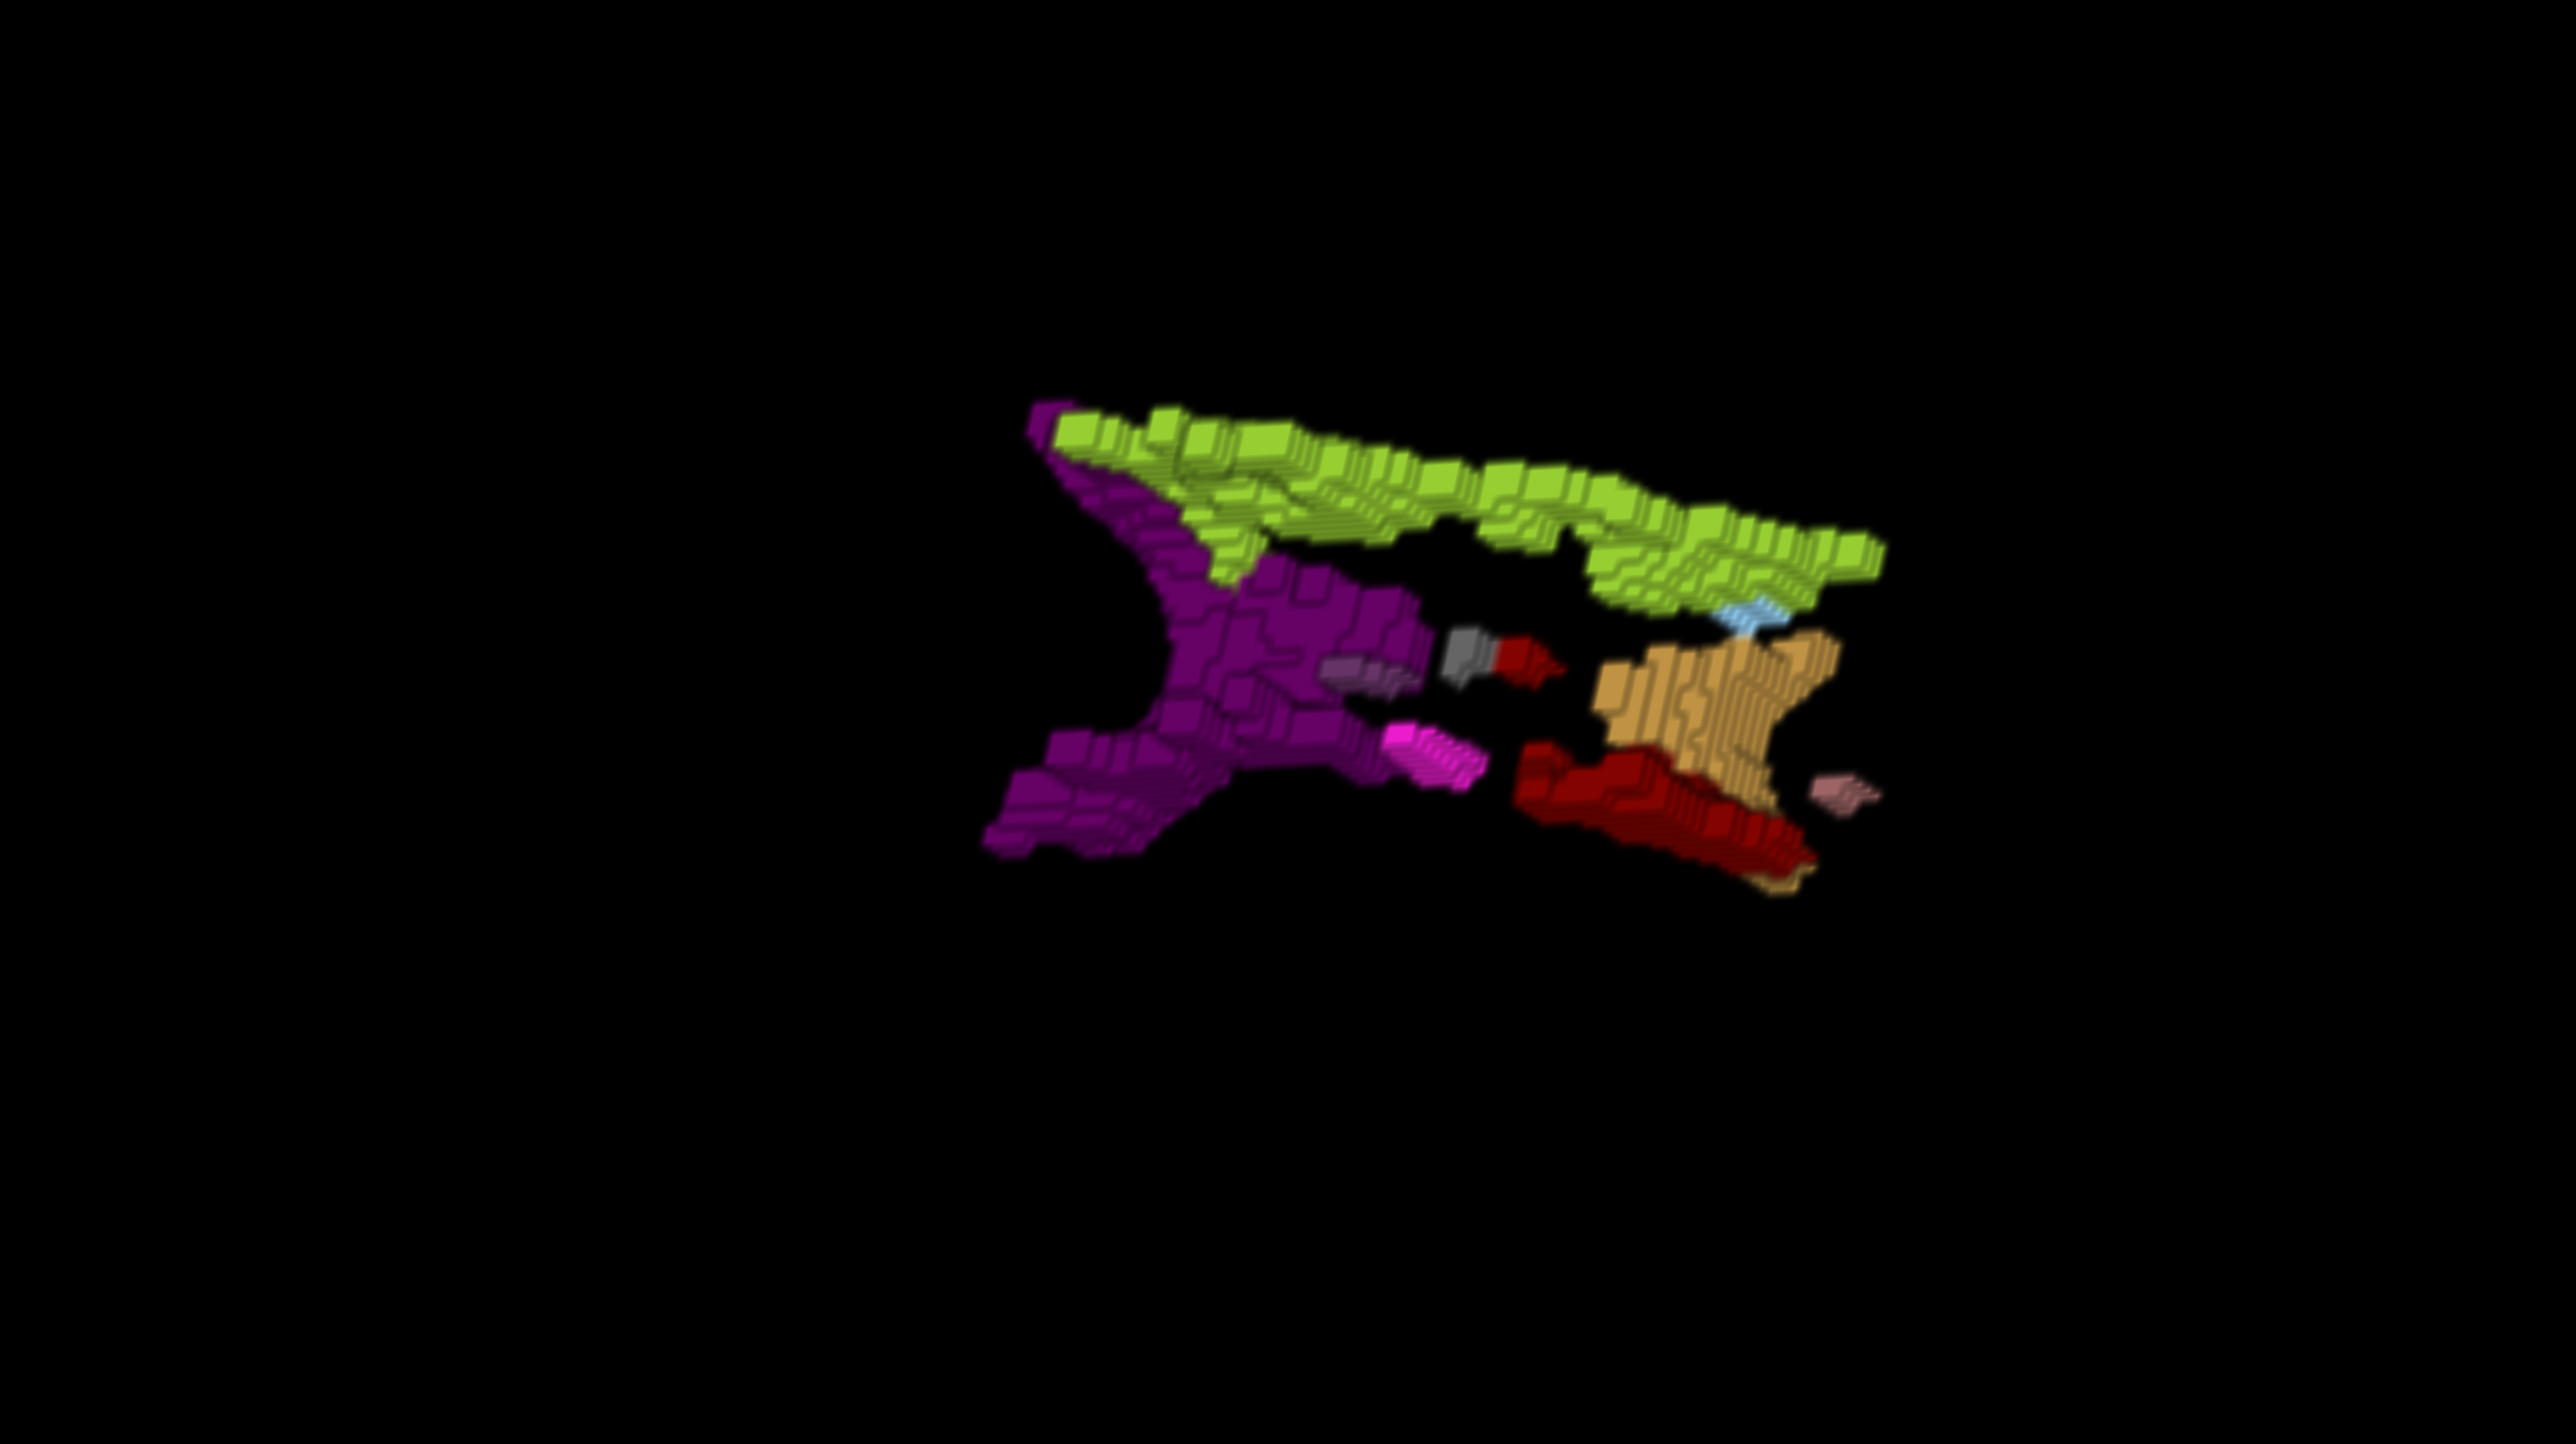
\includegraphics[width=1\linewidth]{img/regions/fa_regions.png}
      \caption{Expanded \textit{corpus callosum} clustered by FA similarity.}
      \label{fig:fa-regions}
    \end{figure}

    \newpage
    \subsubsection{RD}
    \begin{figure}[!ht]
      \centering

      \begin{subfigure}[t]{.49\textwidth}
        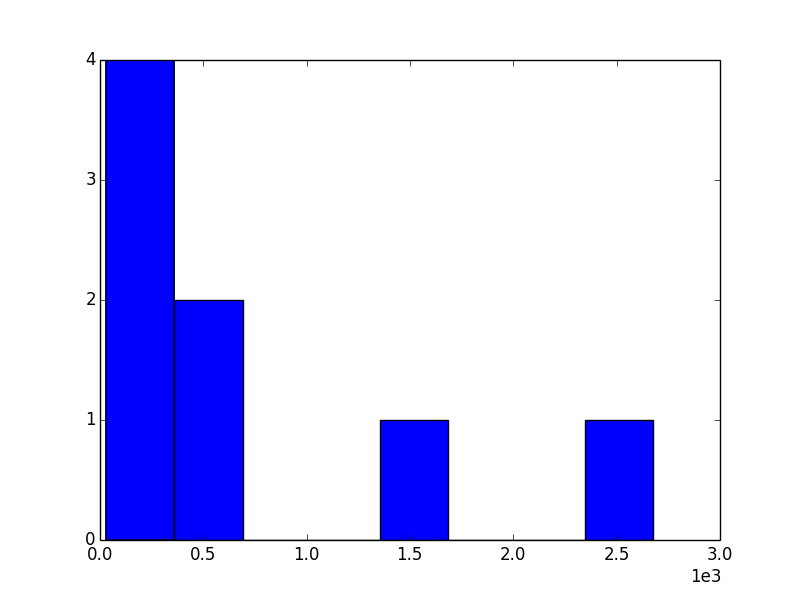
\includegraphics[width=1\linewidth]{img/histograms/rd_clustered_fa_mask_region_sizes_hist.png}
        \caption{Cluster size distribution histogram (Voxel count X Cluster count).}
        \label{subfig:fa_hist_region}
      \end{subfigure}\hfill%
      \begin{subfigure}[t]{.49\textwidth}
        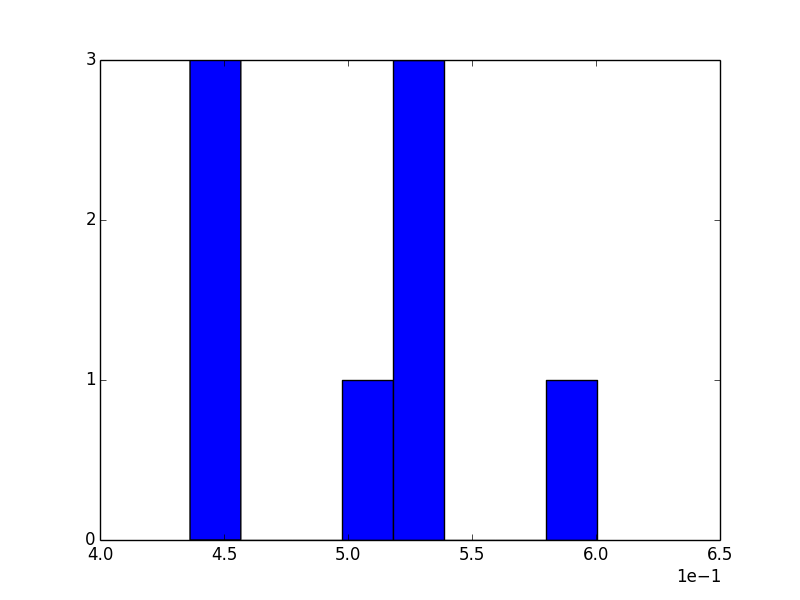
\includegraphics[width=1\linewidth]{img/histograms/rd_clustered_fa_mask_fa_means_hist.png}
        \caption{Histogram for FA mean frequency (Cluster count X FA mean).}
        \label{subfig:fa_hist_fa}
      \end{subfigure}\hfill\\
      \begin{subfigure}[t]{.49\textwidth}
        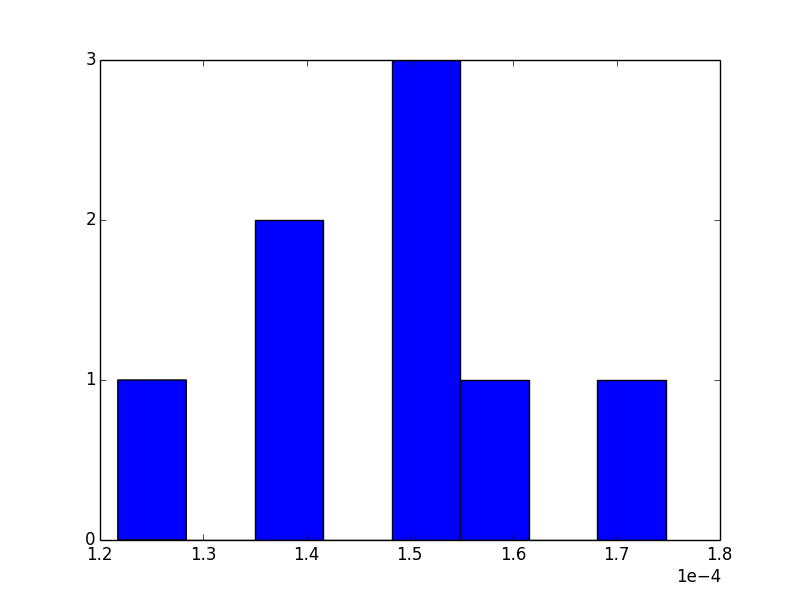
\includegraphics[width=1\linewidth]{img/histograms/rd_clustered_fa_mask_md_means_hist.png}
        \caption{Histogram for MD mean frequency (Cluster count X MD mean).}
        \label{subfig:fa_hist_md}
      \end{subfigure}\hfill%
      \begin{subfigure}[t]{.49\textwidth}
        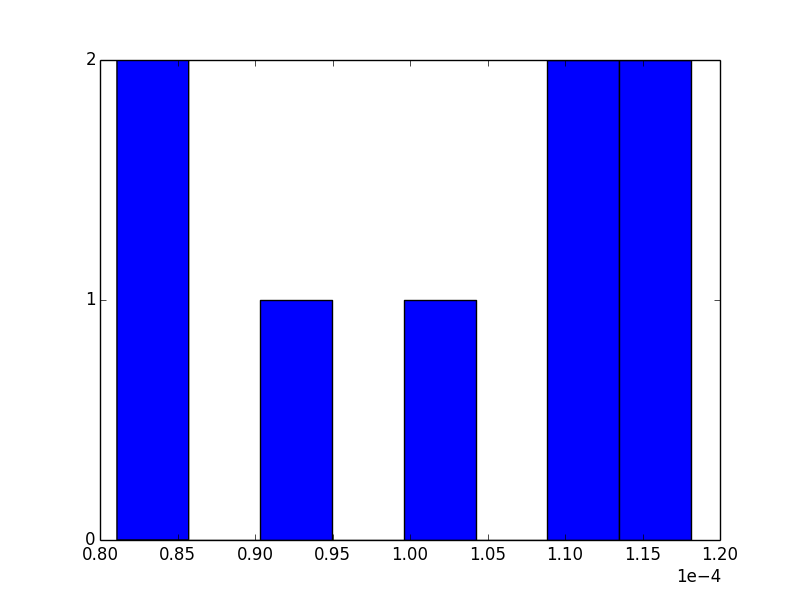
\includegraphics[width=1\linewidth]{img/histograms/rd_clustered_fa_mask_rd_means_hist.png}
        \caption{Histogram for RD mean frequency (Cluster count X RD mean).}
        \label{subfig:fa_hist_rd}
      \end{subfigure}\hfill\\
      \begin{subfigure}[t]{.49\textwidth}
        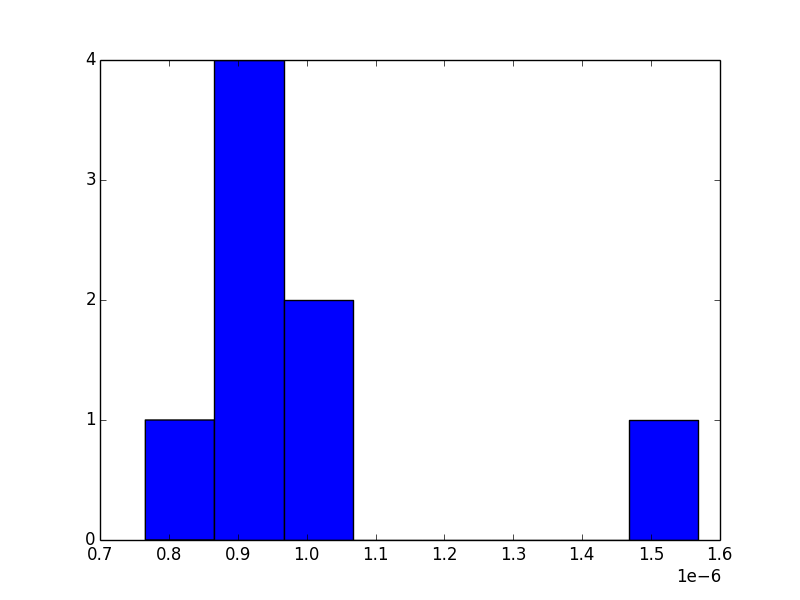
\includegraphics[width=1\linewidth]{img/histograms/rd_clustered_fa_mask_tc_means_hist.png}
        \caption{Histogram for TC mean frequency (Cluster count X TC mean).}
        \label{subfig:fa_hist_tc}
      \end{subfigure}\hfill%
      \begin{subfigure}[t]{.49\textwidth}
        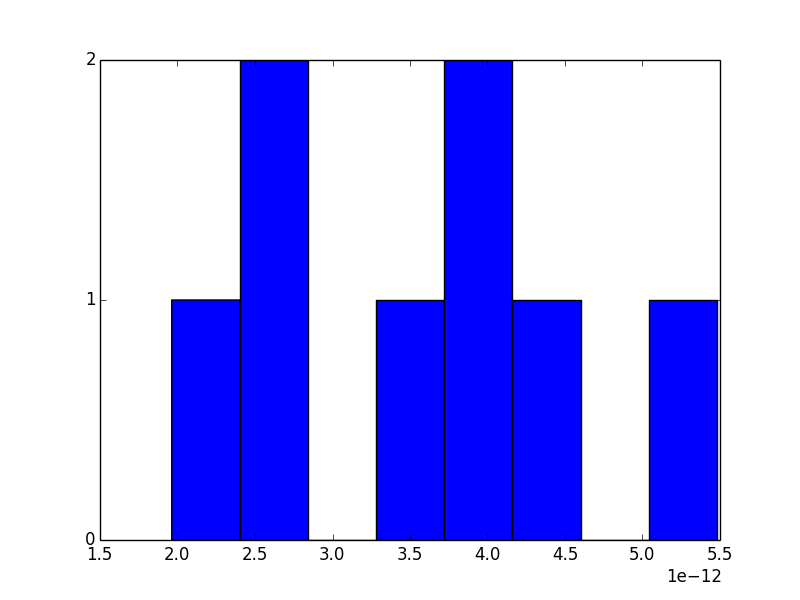
\includegraphics[width=1\linewidth]{img/histograms/rd_clustered_fa_mask_tv_means_hist.png}
        \caption{Histogram for TV mean frequency (Cluster count X TV mean).}
        \label{subfig:fa_hist_tv}
      \end{subfigure}\hfill

      \caption{Histograms for statistics distribution when clustered by RD values.}
      \label{fig:fa-histograms}
    \end{figure}

    This type of clusterization grouped voxels with RD values which don't differ no more then 0.000029 (standard deviation from the entire region \ref{subsec:fa-threshold}) taking 7m36.263s to get computed and another 0m33.861s to generate the statistics.

    Those statistics refers to the following colored regions on \ref{fig:rd-regions}.

    \begin{figure}[!ht]
      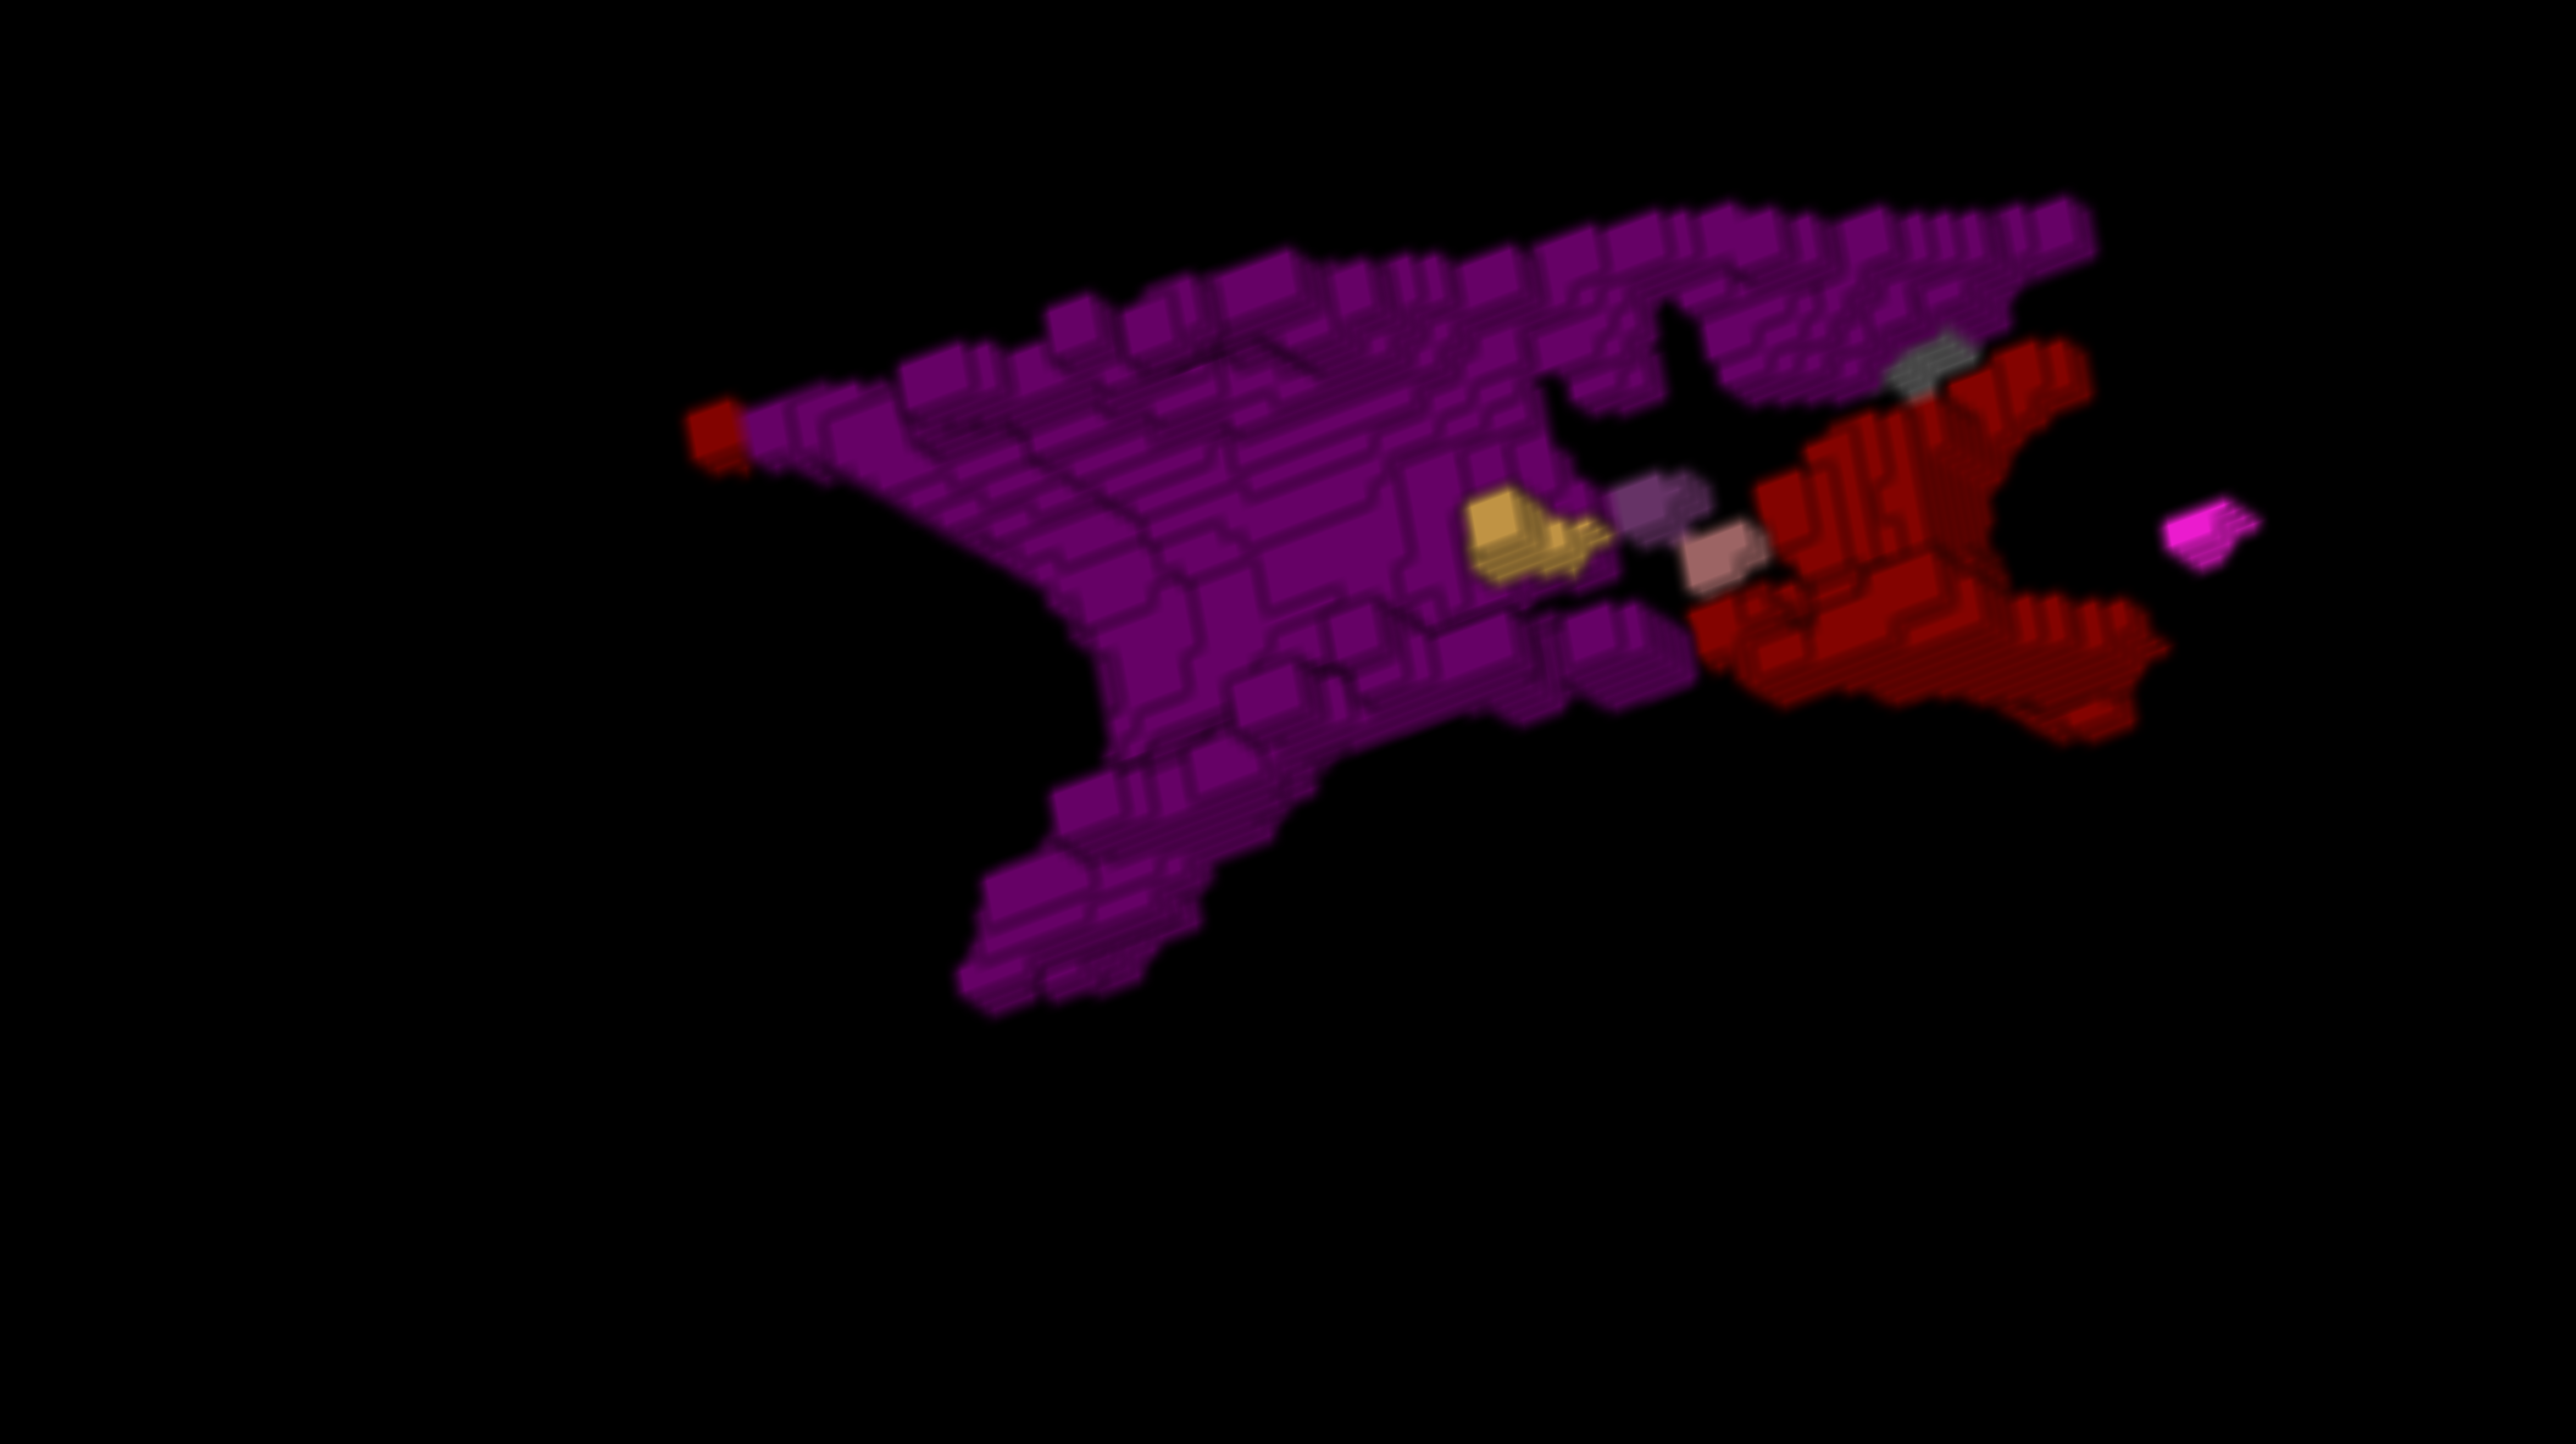
\includegraphics[width=1\linewidth]{img/regions/rd_regions.png}
      \caption{Expanded \textit{corpus callosum} clustered by RD similarity.}
      \label{fig:rd-regions}
    \end{figure}

    \newpage
    \subsubsection{TC}
    \begin{figure}[!ht]
      \centering

      \begin{subfigure}[t]{.49\textwidth}
        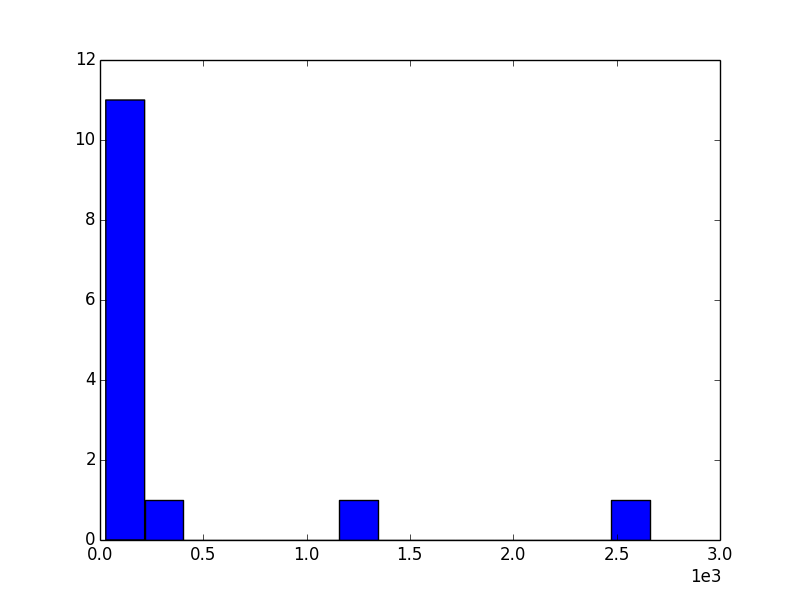
\includegraphics[width=1\linewidth]{img/histograms/tc_clustered_fa_mask_region_sizes_hist.png}
        \caption{Cluster size distribution histogram (Voxel count X Cluster count).}
        \label{subfig:fa_hist_region}
      \end{subfigure}\hfill%
      \begin{subfigure}[t]{.49\textwidth}
        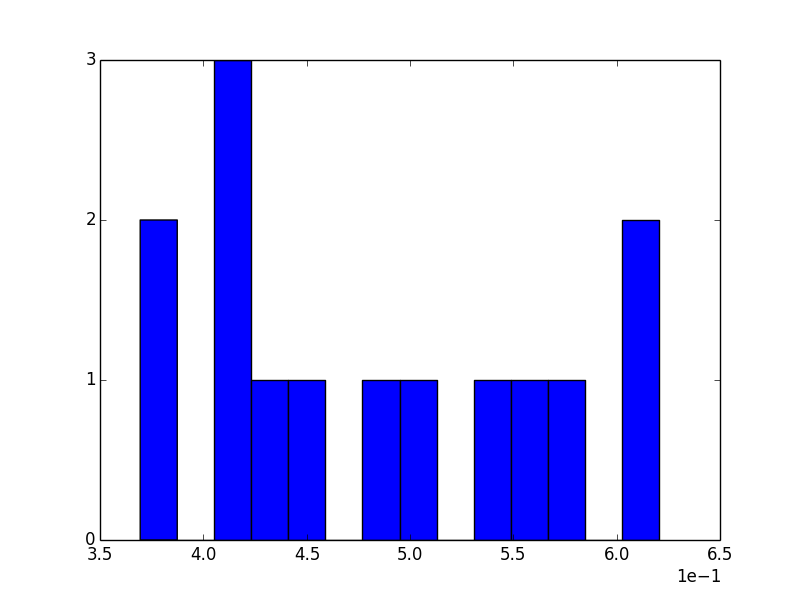
\includegraphics[width=1\linewidth]{img/histograms/tc_clustered_fa_mask_fa_means_hist.png}
        \caption{Histogram for FA mean frequency (Cluster count X FA mean).}
        \label{subfig:fa_hist_fa}
      \end{subfigure}\hfill\\
      \begin{subfigure}[t]{.49\textwidth}
        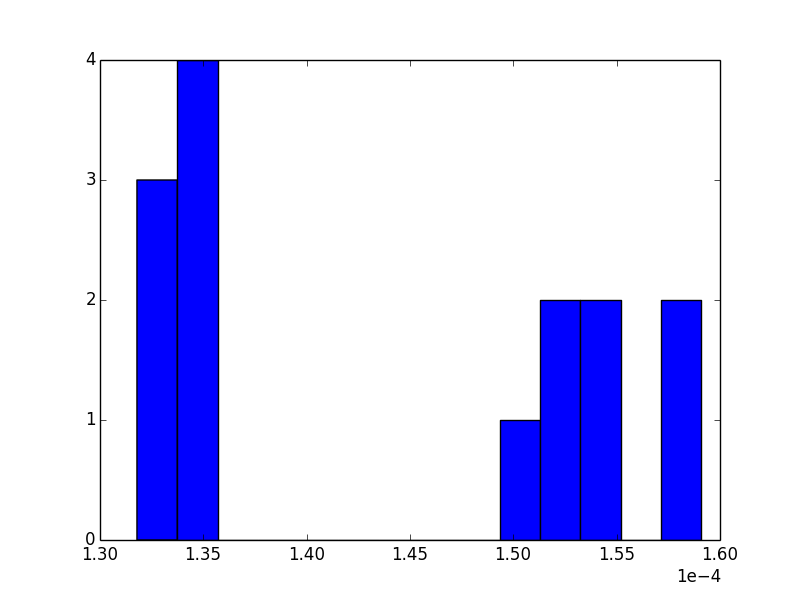
\includegraphics[width=1\linewidth]{img/histograms/tc_clustered_fa_mask_md_means_hist.png}
        \caption{Histogram for MD mean frequency (Cluster count X MD mean).}
        \label{subfig:fa_hist_md}
      \end{subfigure}\hfill%
      \begin{subfigure}[t]{.49\textwidth}
        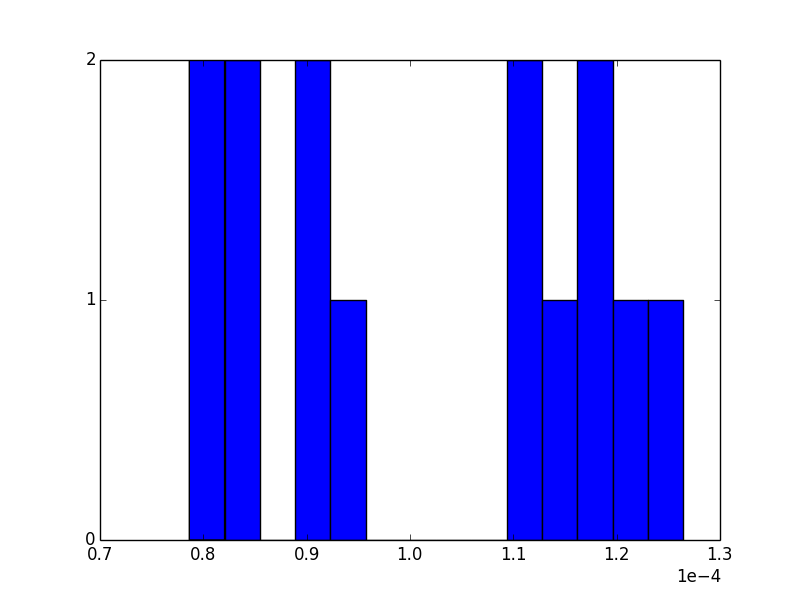
\includegraphics[width=1\linewidth]{img/histograms/tc_clustered_fa_mask_rd_means_hist.png}
        \caption{Histogram for RD mean frequency (Cluster count X RD mean).}
        \label{subfig:fa_hist_rd}
      \end{subfigure}\hfill\\
      \begin{subfigure}[t]{.49\textwidth}
        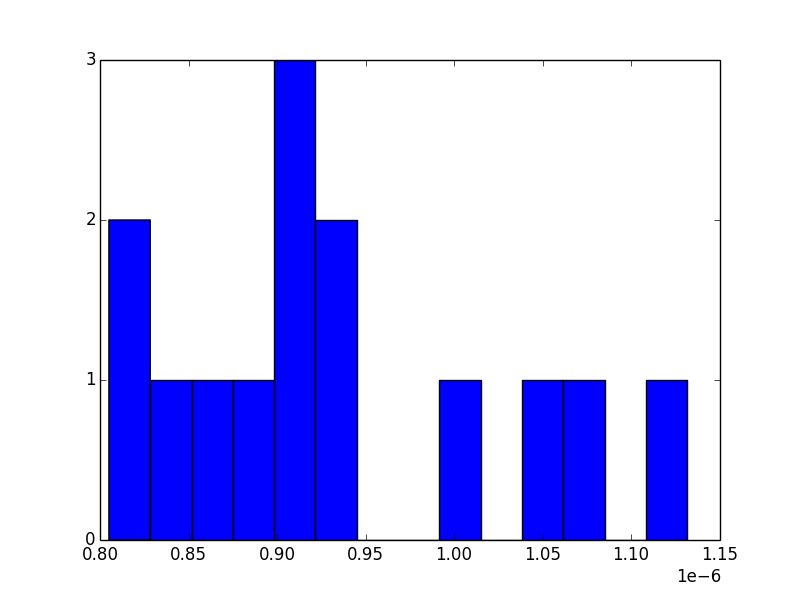
\includegraphics[width=1\linewidth]{img/histograms/tc_clustered_fa_mask_tc_means_hist.png}
        \caption{Histogram for TC mean frequency (Cluster count X TC mean).}
        \label{subfig:fa_hist_tc}
      \end{subfigure}\hfill%
      \begin{subfigure}[t]{.49\textwidth}
        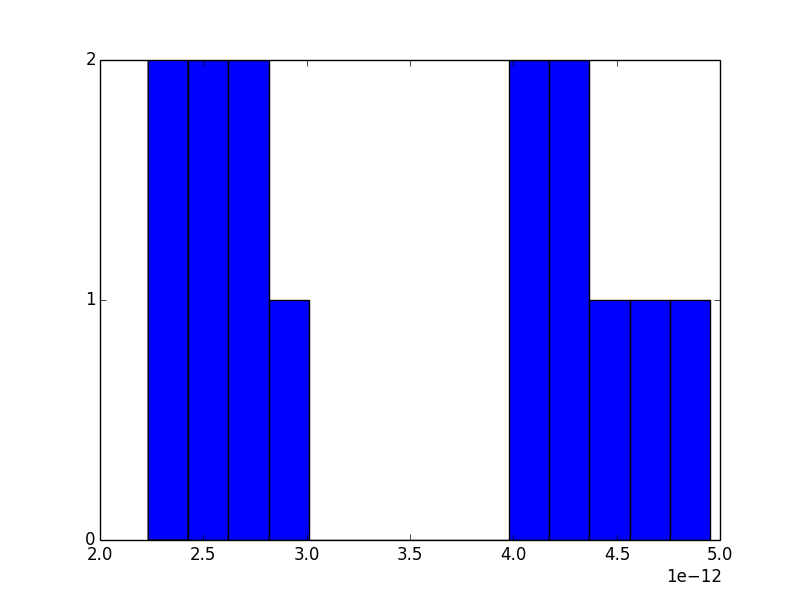
\includegraphics[width=1\linewidth]{img/histograms/tc_clustered_fa_mask_tv_means_hist.png}
        \caption{Histogram for TV mean frequency (Cluster count X TV mean).}
        \label{subfig:fa_hist_tv}
      \end{subfigure}\hfill

      \caption{Histograms for statistics distribution when clustered by TC values.}
      \label{fig:fa-histograms}
    \end{figure}

    This type of clusterization grouped voxels with FA values which don't differ no more then 0.0000004 (standard deviation from the entire region \ref{subsec:fa-threshold}) taking 17m4.241s to get computed and another 0m31.865s to generate the statistics.

    Those statistics refers to the following colored regions on \ref{fig:tc-regions}.

    \begin{figure}[!ht]
      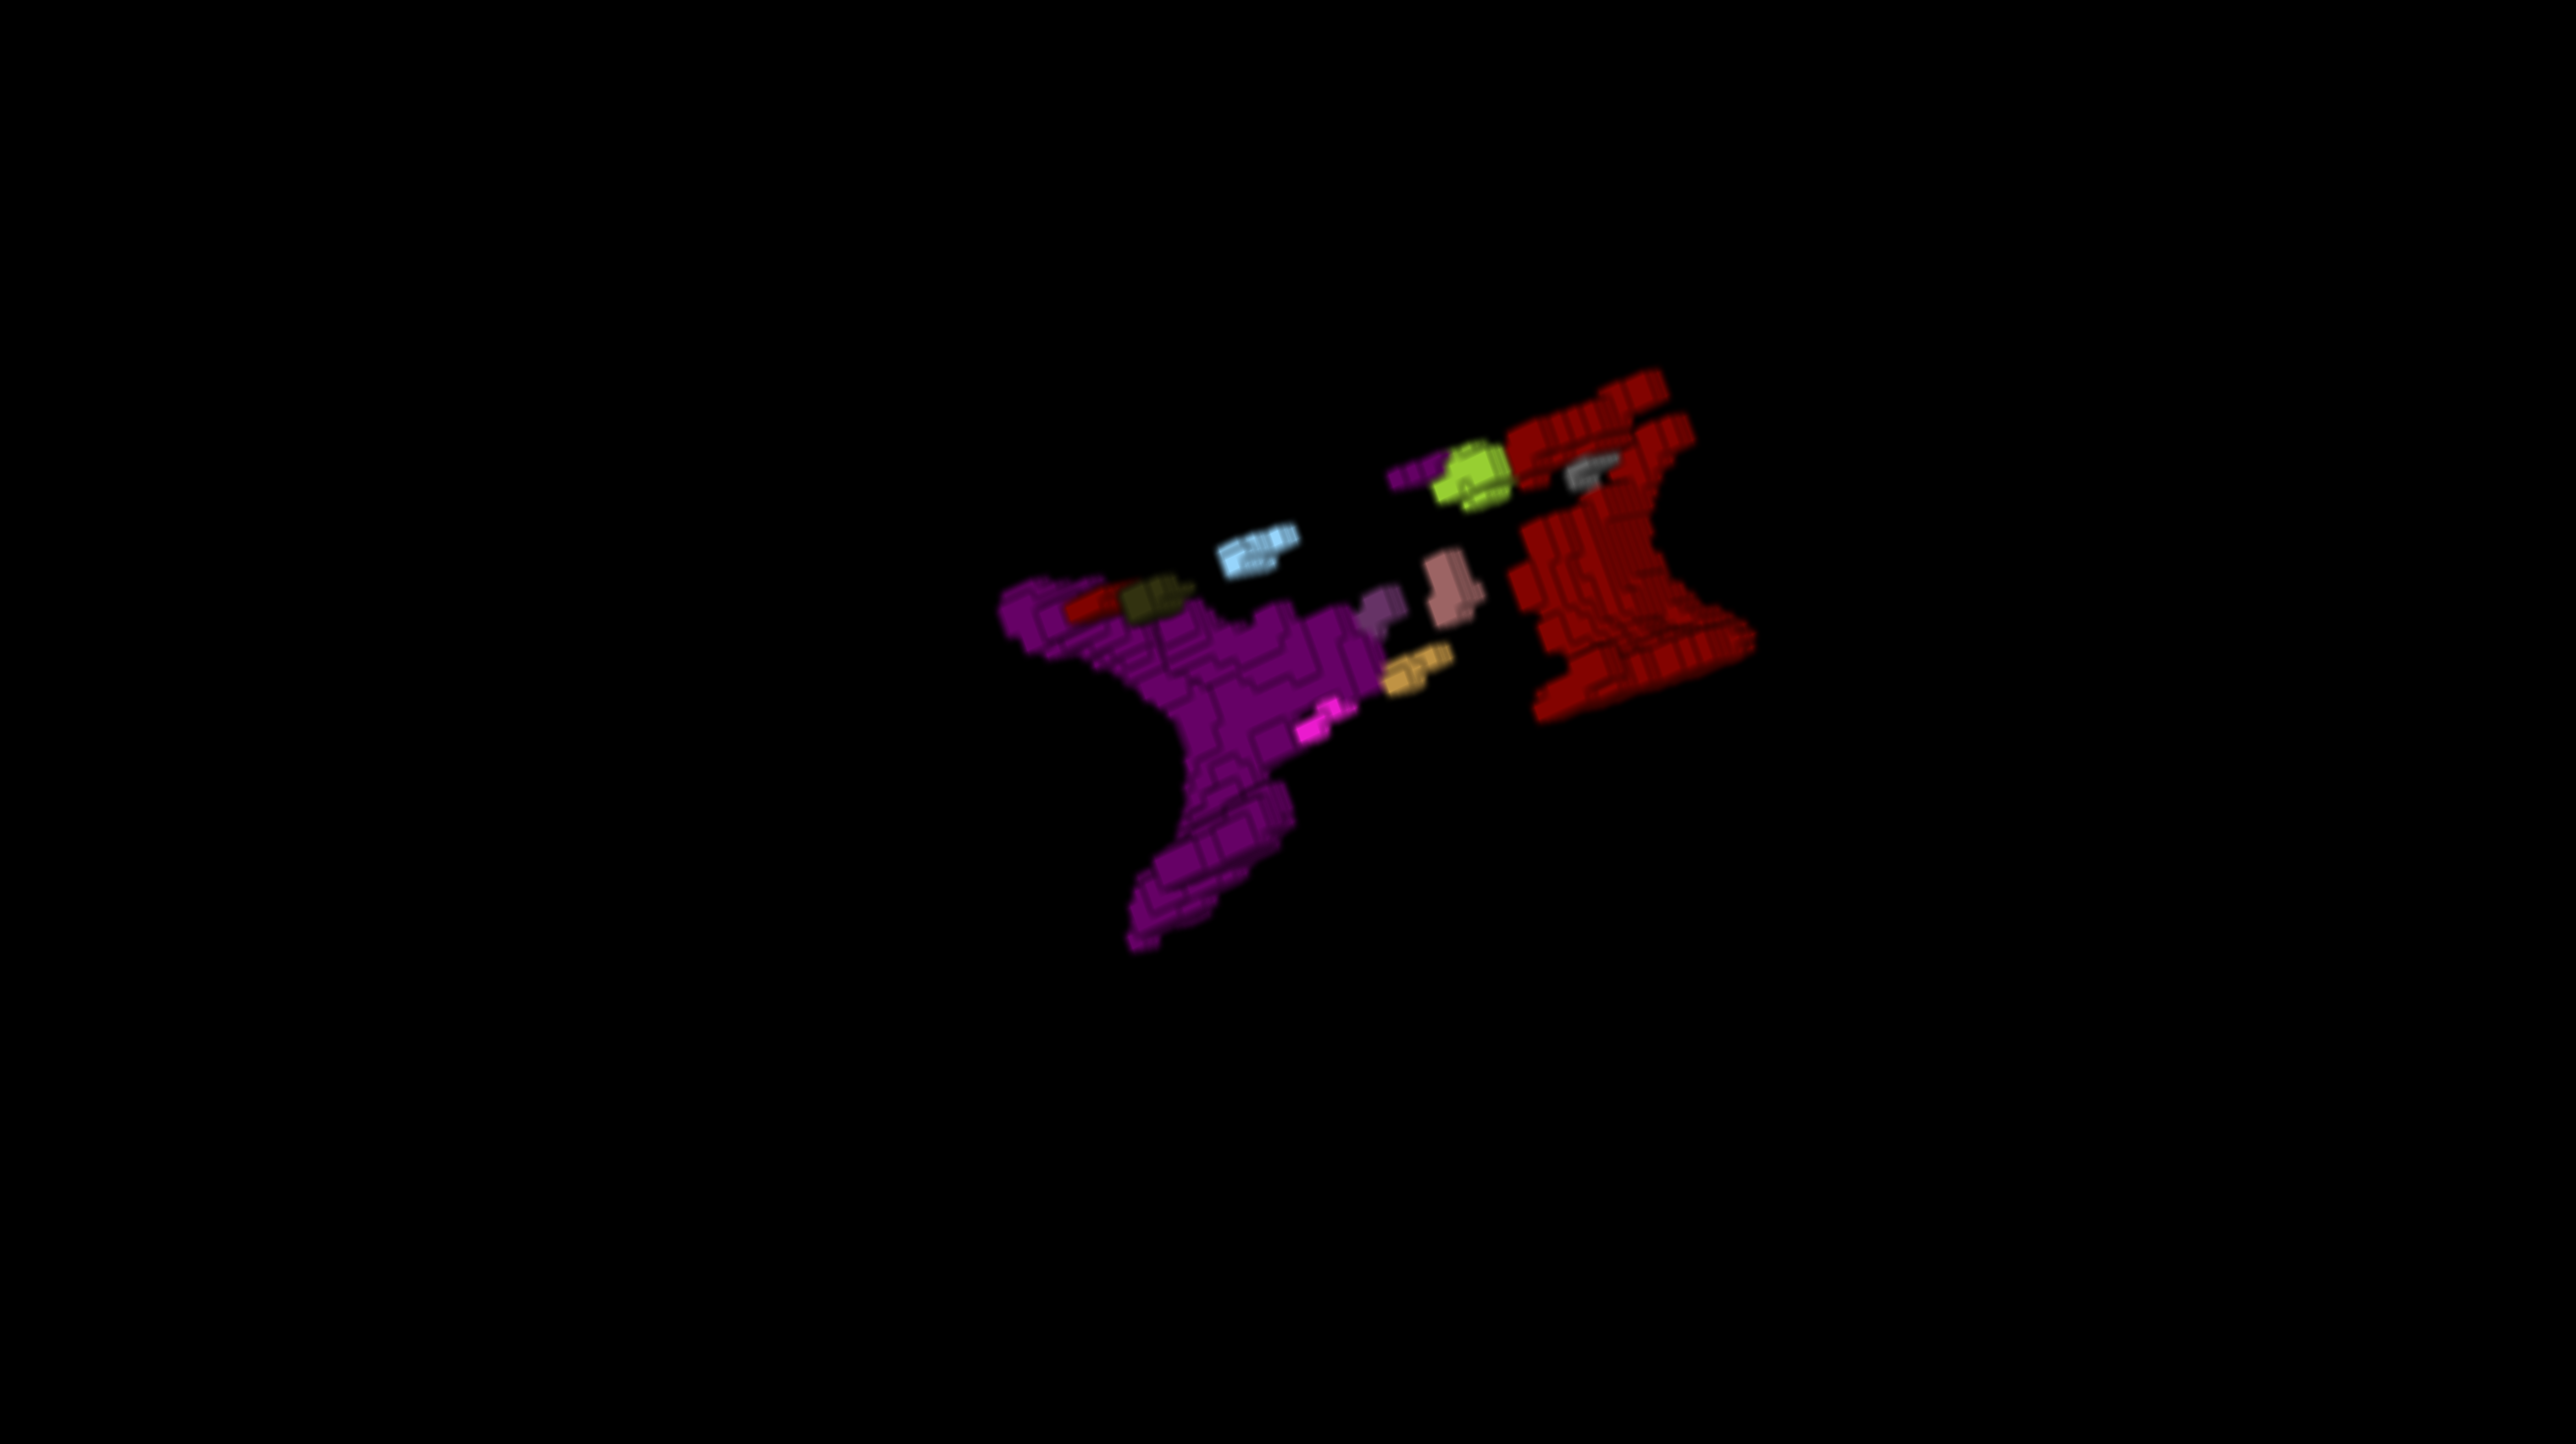
\includegraphics[width=1\linewidth]{img/regions/tc_regions.png}
      \caption{Expanded \textit{corpus callosum} clustered by TC similarity.}
      \label{fig:tc-regions}
    \end{figure}

    \newpage
    \subsubsection{TV}
    \begin{figure}[!ht]
      \centering

      \begin{subfigure}[t]{.49\textwidth}
        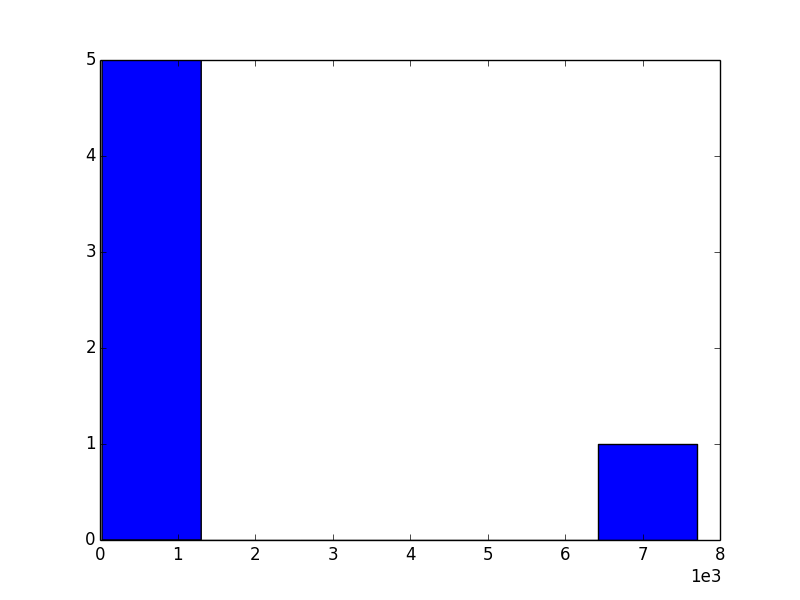
\includegraphics[width=1\linewidth]{img/histograms/tv_clustered_fa_mask_region_sizes_hist.png}
        \caption{Cluster size distribution histogram (Voxel count X Cluster count).}
        \label{subfig:fa_hist_region}
      \end{subfigure}\hfill%
      \begin{subfigure}[t]{.49\textwidth}
        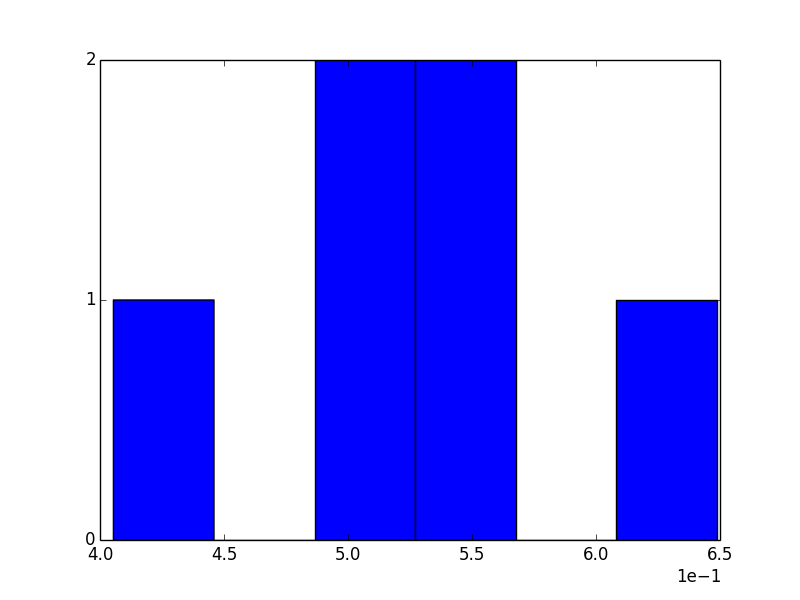
\includegraphics[width=1\linewidth]{img/histograms/tv_clustered_fa_mask_fa_means_hist.png}
        \caption{Histogram for FA mean frequency (Cluster count X FA mean).}
        \label{subfig:fa_hist_fa}
      \end{subfigure}\hfill\\
      \begin{subfigure}[t]{.49\textwidth}
        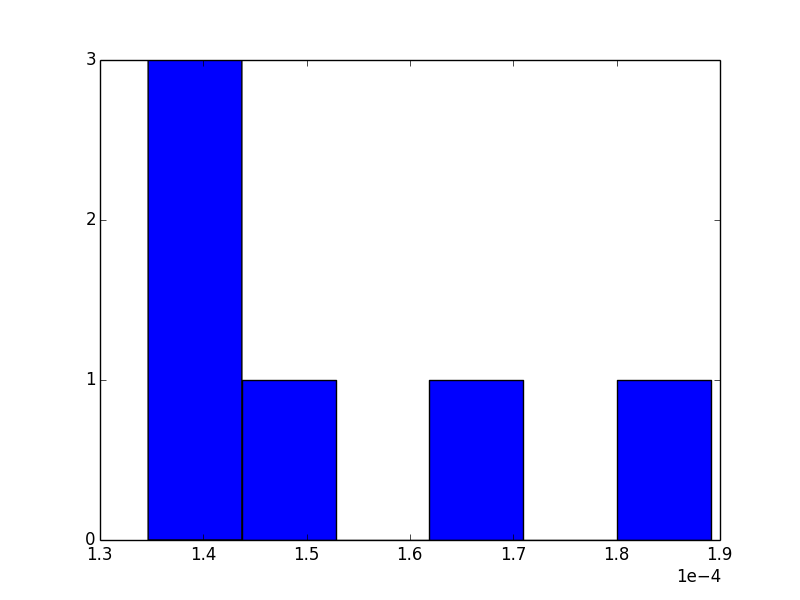
\includegraphics[width=1\linewidth]{img/histograms/tv_clustered_fa_mask_md_means_hist.png}
        \caption{Histogram for MD mean frequency (Cluster count X MD mean).}
        \label{subfig:fa_hist_md}
      \end{subfigure}\hfill%
      \begin{subfigure}[t]{.49\textwidth}
        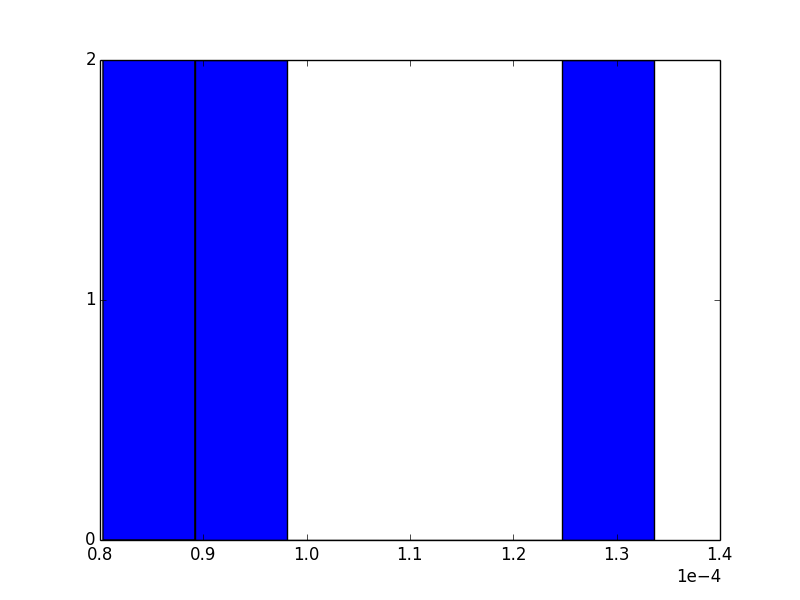
\includegraphics[width=1\linewidth]{img/histograms/tv_clustered_fa_mask_rd_means_hist.png}
        \caption{Histogram for RD mean frequency (Cluster count X RD mean).}
        \label{subfig:fa_hist_rd}
      \end{subfigure}\hfill\\
      \begin{subfigure}[t]{.49\textwidth}
        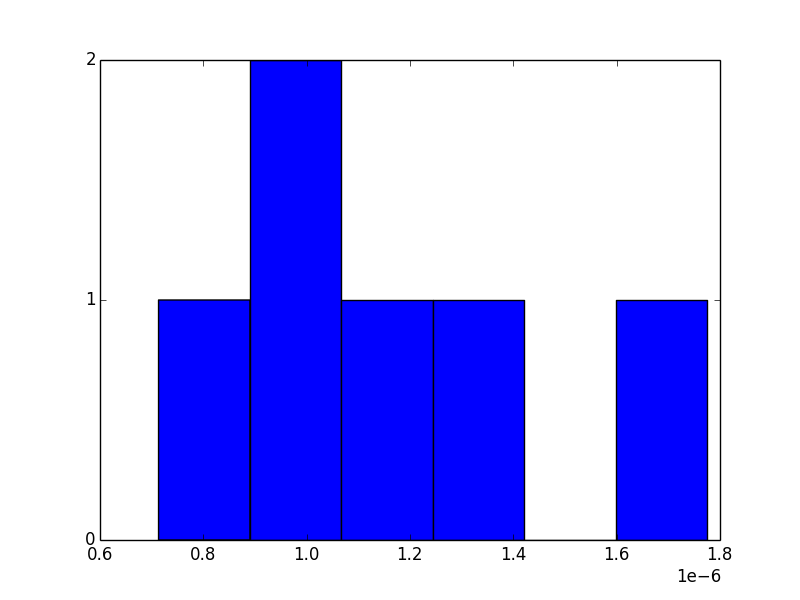
\includegraphics[width=1\linewidth]{img/histograms/tv_clustered_fa_mask_tc_means_hist.png}
        \caption{Histogram for TC mean frequency (Cluster count X TC mean).}
        \label{subfig:fa_hist_tc}
      \end{subfigure}\hfill%
      \begin{subfigure}[t]{.49\textwidth}
        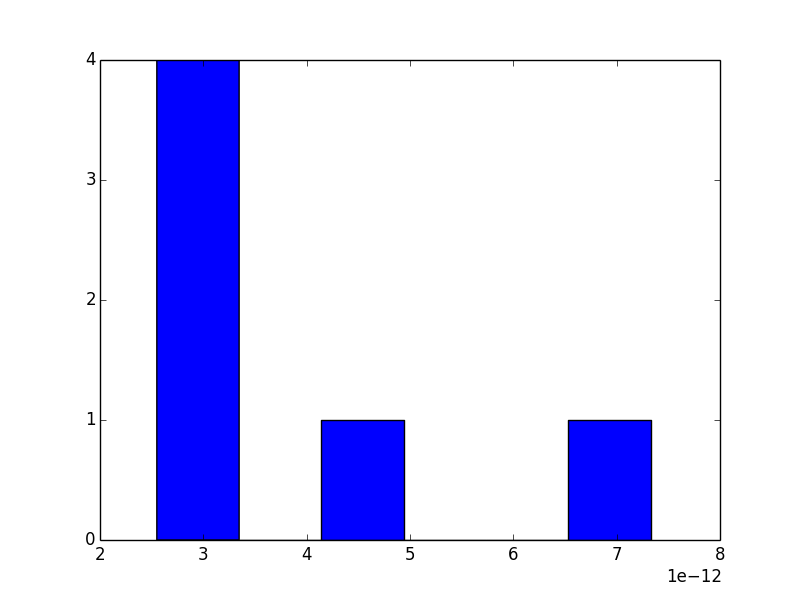
\includegraphics[width=1\linewidth]{img/histograms/tv_clustered_fa_mask_tv_means_hist.png}
        \caption{Histogram for TV mean frequency (Cluster count X TV mean).}
        \label{subfig:fa_hist_tv}
      \end{subfigure}\hfill

      \caption{Histograms for statistics distribution when clustered by TV values.}
      \label{fig:fa-histograms}
    \end{figure}

    This type of clusterization grouped voxels with FA values which don't differ no more then 0.00000000001 taking 7m55.727s to get computed and another 0m48.003s to generate the statistics.

    Those statistics refers to the following colored regions on \ref{fig:tv-regions}.

    \begin{figure}[!ht]
      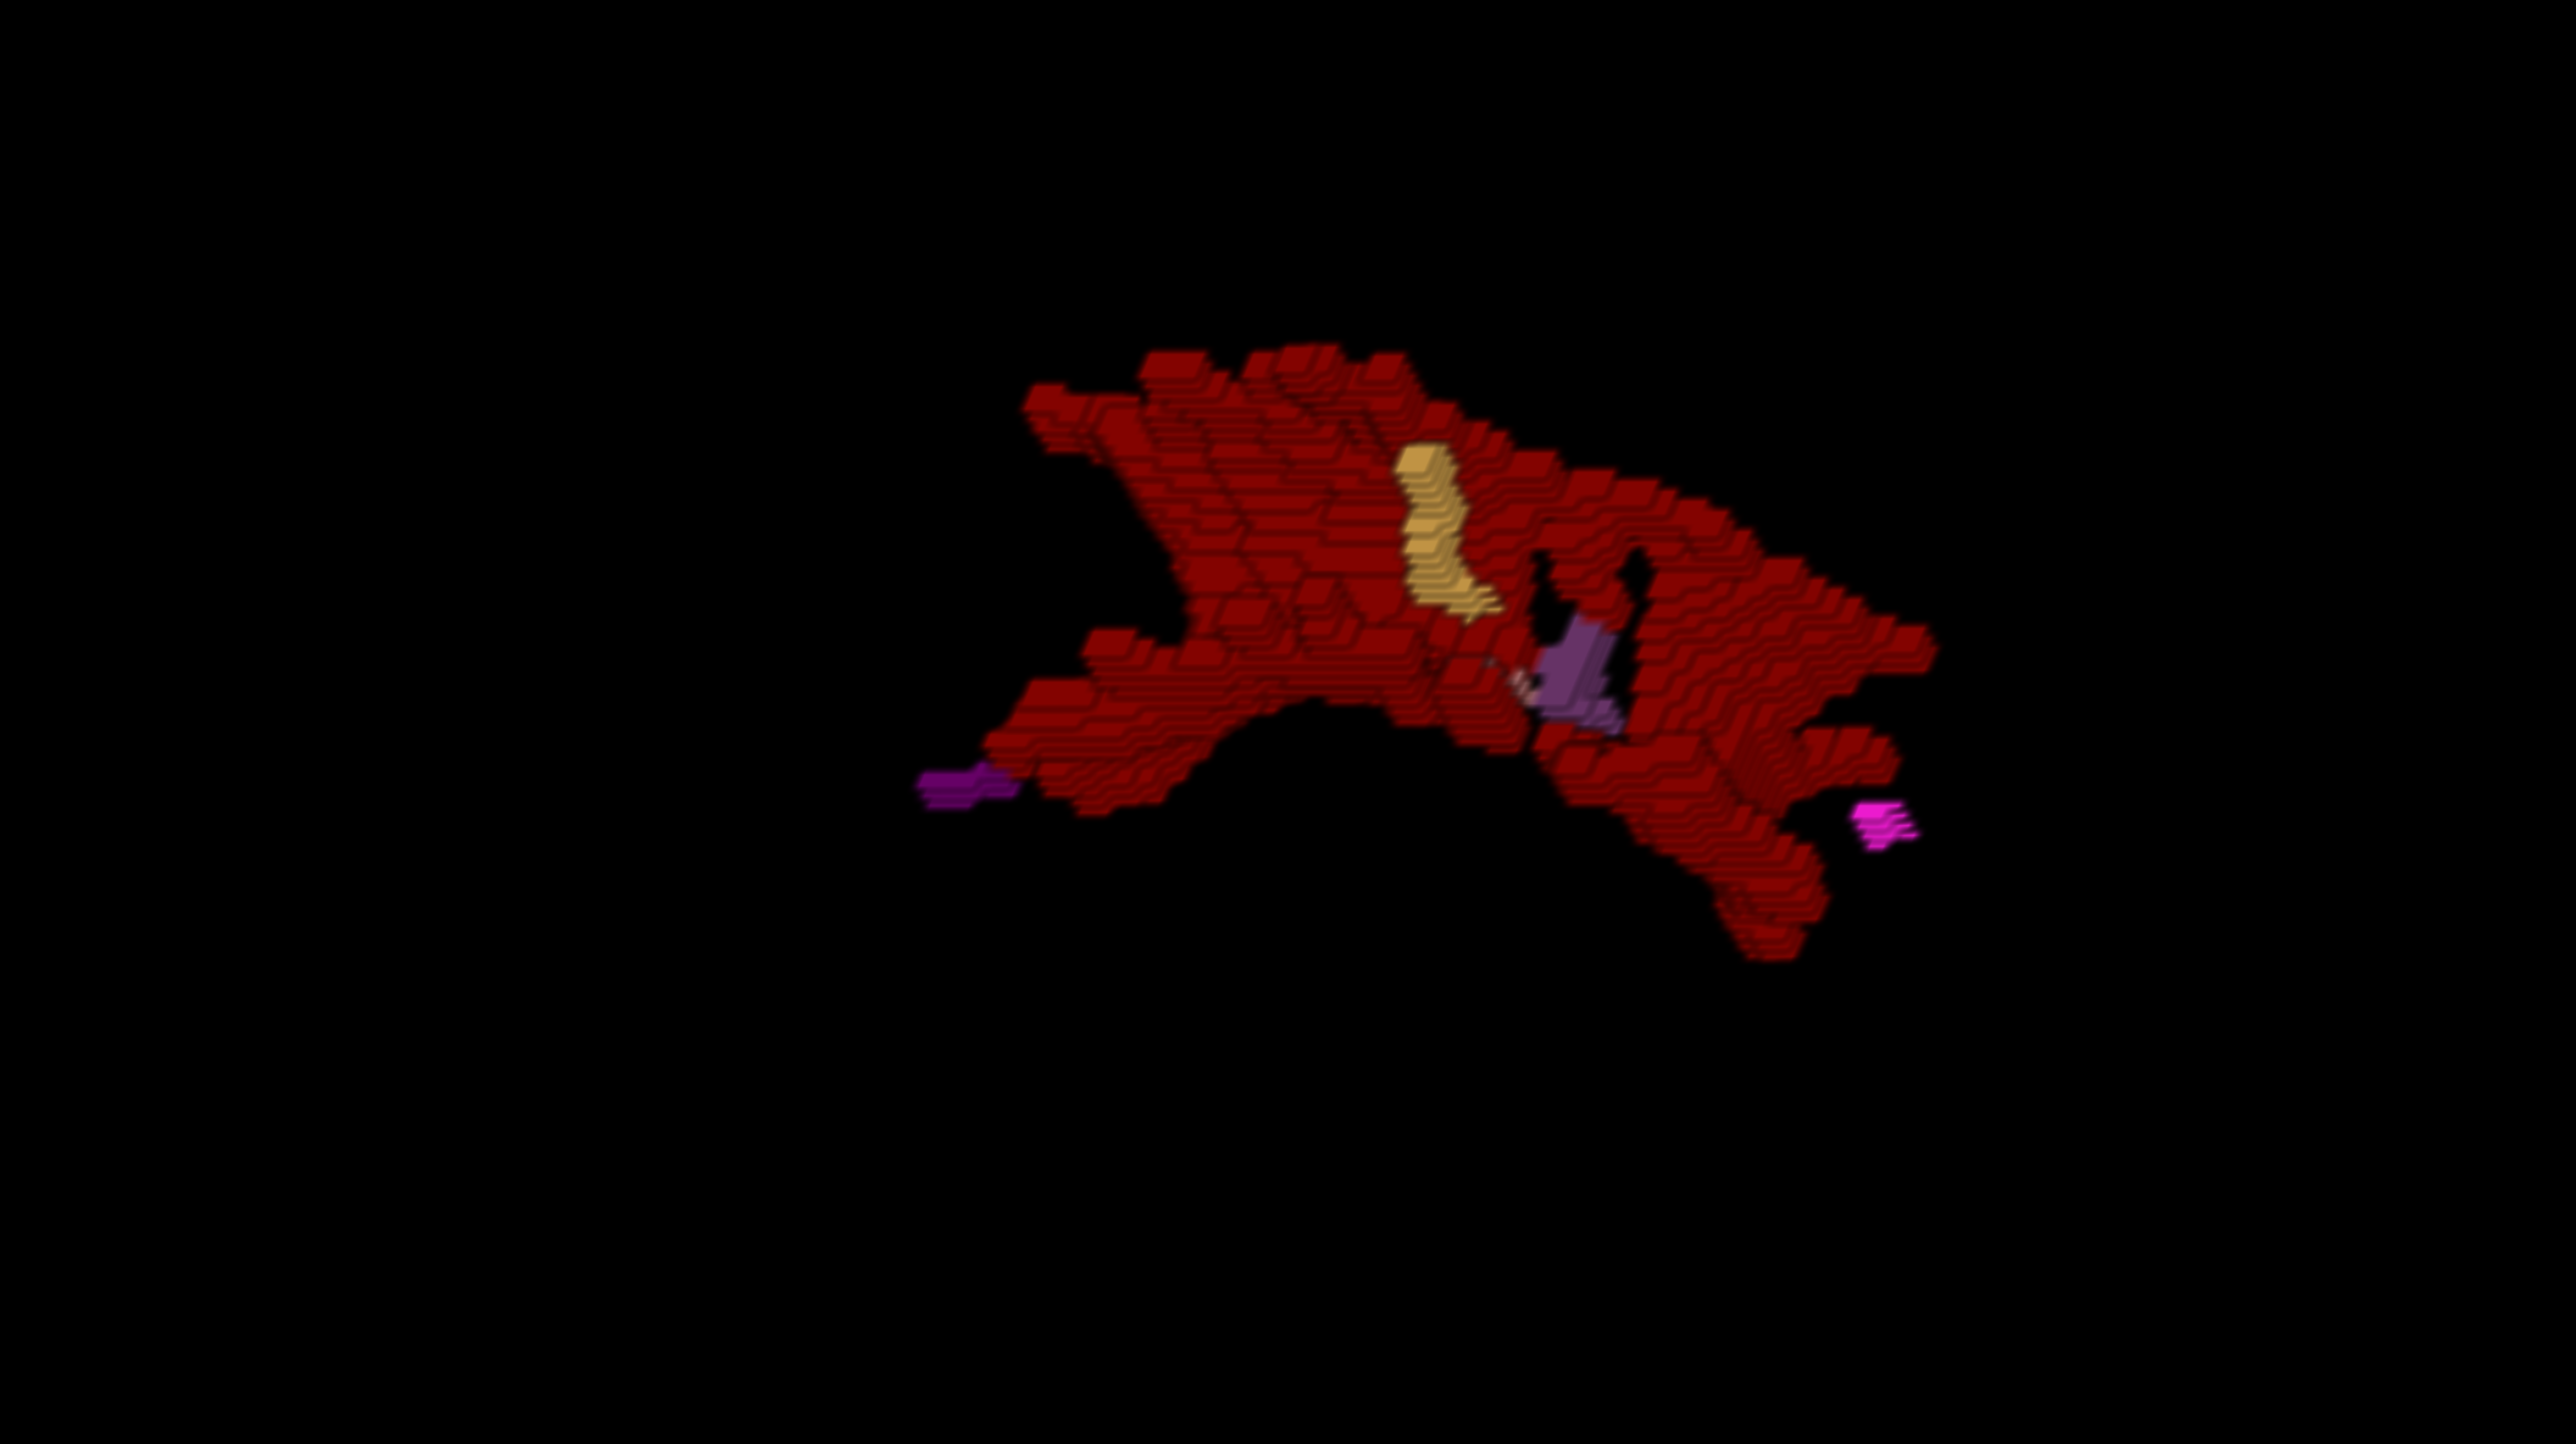
\includegraphics[width=1\linewidth]{img/regions/tv_regions.png}
      \caption{Expanded \textit{corpus callosum} clustered by RD similarity.}
      \label{fig:tv-regions}
    \end{figure}

\section{Phantom sketch}

\chapter{Discussion}

\end{document}